\chapter{Méthodes}

J'ai utilisé la base de donnée présentée dans la partie\ref{lab:bdd} pour évaluer les performances des techniques de correction du mouvement respiratoire présentés dans le chapitre \ref{lab:corrMvt}. 

Les techniques de correction du mouvement implémentées sont les suivantes :

\begin{enumerate}
 \item Correction pendant la reconstruction par modification de la matrice système (voir section \ref{lab:corrMatSyst})
 \item Correction post-reconstruction par recalage des images prises à différents instants du cycle (voir section \ref{lab:corrPostRecon})
\end{enumerate}

Elles sont comparées avec les images non corrigées et des images statiques (qui représentent une correction parfaite).

Dans le cas présent, l'objectif est d'évaluer les performances des techniques de correction du mouvement sur la détection des lésions de faible contraste et faible diamètre. Pour cela, les performances d'un système de détection automatique seront mesurées à l'aide des courbes F-ROC.

\section{Système CAD} % 11.1

Le système CAD que nous utilisons a été développé à l'origine pendant les travaux de thèse de Sandrine Tomeï ainsi que mes travaux de master~\cite{tomei2008automatic,lartizien2010impact}. Nous l'avons amélioré et adapté aux besoins de cette étude, notamment en développant les mesures de performances.


Le CAD utilise des informations fréquentielles obtenue par décomposition non décimée des images en ondelettes Biorthogonale 4.4. Ces données sont utilisées par le système de classification basé sur un SVM travaillant voxel par voxel. Une étape de réduction des faux positifs est ajoutée par la suite.
Étant donné le faible nombre de tumeurs présentes dans les organes considérés, la base d'apprentissage est générée à partir des images utilisées pour la base de test. 

\subsection{Vecteur de Caractéristiques}

Nous avons choisi d’utiliser une décomposition en ondelettes 3D non décimée par banc de filtres. Dans le cas tridimensionnel, la décomposition par banc de filtre est résumé par la Figure \ref{fig:ondelettes}. L’image de départ est filtrée séparément dans les trois directions de l’espace par un filtre fréquentiel passe-haut correspondant à la fonction d’ondelettes (noté $H$) et passe-bas correspondant à la fonction d’échelle (noté $L$). 

Ainsi sept images de détails (HHH, LLH, \dots) et une image d’approximation (LLL) sont produites pour chaque niveau $j$ de décomposition. Les huit images du niveau suivant $j+1$ sont générées de la même manière, mais en considérant l’image d’approximation $LLL_j$ du niveau précédent comme image de départ. Les caractéristiques des images, rassemblées dans un vecteur descripteur de taille $8\times j$, correspondent ici à l’ensemble de ces coefficients pour chaque voxel  de l’image. 

\begin{figure}
 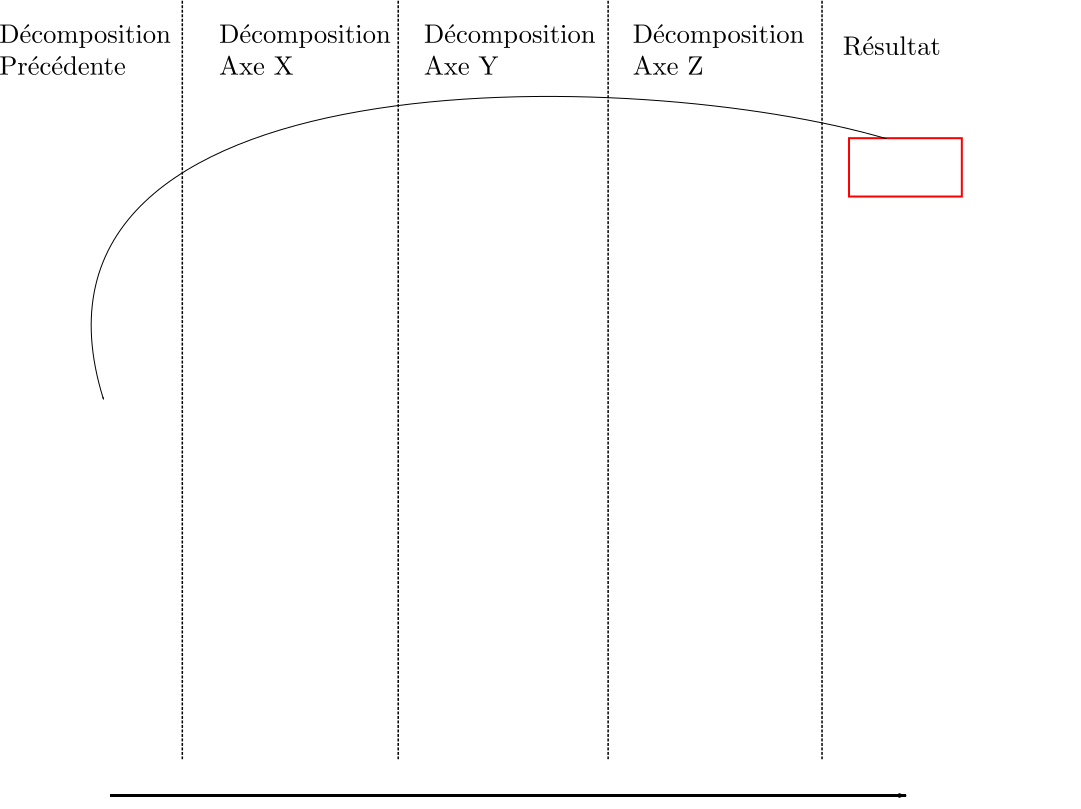
\includegraphics[width=15cm]{images/decompHotell}
 \caption{Décomposition en ondelettes par banc de filtres : Chaque image est filtrée selon les 3 dimensions pour obtenir les coefficients d'ondelettes et d'échelle de chaque voxel de l'image.}
 \label{fig:ondelettes}
\end{figure}


\subsection{Génération de la base d'apprentissage}
Les données générées par la décomposition en ondelettes de chaque image se présentent sous la forme de volumes 4D, indiquant pour chaque voxels de l'image 3D l'ensemble des coefficients associés.

La base d'apprentissage sert à entraîner le classifieur dans un processus de classification supervisée, en lui fournissant un ensemble d'exemples avec leur classes associées (voir figure \ref{fig:fonctClassif}) page \pageref{fig:fonctClassif}).

La génération de cette base demande l'extraction de points de la classe ``pathologique'', et de la classe ``sain''. Les points correspondants à la classe pathologique sont extraits des centres de chaque tumeur de chaque image de la base pour l'organe considéré. Les points de la classe ``sain'' sont extraits de manière aléatoire dans les volumes de toutes les images (hors tumeurs). Pour des raisons de simplicité d'implémentation, un nombre fixe de points sont extraits de chaque image.

\subsection{Apprentissage de la Machine à Vecteur de Support (SVM)}

Une fois la base de données générée, elle sera fournie en entrée au classifieur SVM (Machine à Vecteur de Support) pour l'apprentissage.

Le principe des SVM est, de trouver l’hyperplan optimal de séparation, qui va maximiser la marge de séparation entre les deux classes ``pathologique''  et ``sain'' (voir \ref{lab:SVM}). Cette marge correspond à la distance à l’hyperplan entre les plus proches vecteurs de caractéristiques appartenant à chacune des classes. La définition de cette marge et donc de l’hyperplan, se fait uniquement à partir de vecteurs de support, qui correspondent à l'enveloppe du groupement de point de l'une des deux classes.

Le SVM va fournir en sortie un modèle décrivant l'hyperplan permettant de séparer les données.

\subsection{Génération des sites présumés}
\label{lab:aggregatsCAD}
Une fois le classifieur entraîné, on lui soumettra les voxels des images pour qu'il les classe. On aura donc en sortie un ensemble de carte de score (une par image), dans lesquelles chaque voxel correspond au score indiqué par le SVM. Ce score est une mesure de distance par rapport à l'hyperplan de séparation dans l'espace des points d'apprentissage, et donne donc une indication de la ``certitude'' du SVM vis-à-vis de sa classification.

Cette carte de score est ensuite seuillée pour fournir une carte binaire, indiquant pour chaque voxel la classe fournie par le SVM. Le mécanisme de sélection du seuil est défini plus tard. 

A cette étape, le résultat est sous forme ``voxels``, et non ''région''. Nous avons choisit de travailler sur des agrégats de points plutôt que directement sur les voxels car les cartes binarisées sont très bruitées, et donc non directement exploitables. Les voxels ``pathologiques'' sont donc agrégés selon une connexité 26 (3x3x3). Un score est associé à chaque  agrégat, correspondant au score le plus important observé dans l'agrégat.

\subsection{Évaluation du résultat}

Pour évaluer le résultat, nous avons mis au point des règles permettant de classer les agrégats si nous avons accès à la vérité terrain. Ce sont ces algorithmes qui sont utilisés dans les évaluateurs de performance présentés ci-après.

Les agrégats sont classés en LL (Lésion localisée) et NL (Lésion Non Localisée) selon qu'ils peuvent être considérés comme des vrai positifs ou des faux positifs :

Soit $L$ l'ensemble des points de la lésion, $A$ les points correspondant à l'amas candidat.

Les agrégats seront considérés comme des vrai positifs si ils intersectent une tumeur selon les règles suivantes, ou comme de faux positifs sinon. Cependant, si leur taille est inférieure à la taille minimale définie par première règle ($\alpha \times card( L )$), l'amas n'est pas considéré.

\begin{description}
 \item[$card( L \cap A ) > \alpha \times card( L )$] avec $\alpha$ fixé de manière empirique à 0.05 qui fixe la proportion minimale de la tumeur qui doit être présente dans l'amas. Elle permet d'éviter les amas qui intersecteraient la tumeur par accident.
 \item[$card( L \cap A ) > \beta \times card( A )$]  avec $\beta$ fixé de manière empirique à 0.20 limite l'étendue de l'amas en dehors de la tumeur.
\end{description}


\subsection{Résumé}

Ce pseudo-code décrit le CAD, de l'importation des images à l'extraction des lésions potentielles:

\begin{enumerate}
 \item Décomposition des images en ondelettes : Pour chaque voxel de l'image d'origine, on obtient entre 8 et 32 coefficients suivant le niveau de décomposition de l'image, qui correspondent au vecteur de caractéristiques utilisés par le classifieur
 \item Extraction de la base d'apprentissage : Les coefficients des centres de toutes les tumeurs sont extraits des volumes décomposés, et vont former la base d'apprentissage pathologique. Un certain nombre de voxels sont tirés aléatoirement dans les zones normales de chaque images et leur coefficients sont ajoutés à la base saine.
 \item Apprentissage : Le classifieur SVM est entraîné sur cette base d'apprentissage pour générer le modèle qui sera utilisé pour le test.
 \item Tests : Le SVM entraîné est utilisé pour classer chaque voxel contenu dans les organes à évaluer (poumon et foie).
 \item Réduction des Faux-positifs : Les points sont agrégés en composantes connexes (connexité 26 en 3 dimensions).
 \item Évaluation : Si nous avons accès à la vérité terrain, il est possible d'évaluer les performances du CAD en classant les agrégats en LL (Lésion Localisée) et LN (Lésion Non Localisée).
\end{enumerate}



\section{Optimisation des paramètres du système CAD} % 11.2
\label{lab:optim}

Les différentes étapes de l'évaluation des performances nécessitent la fixation d'un grand nombre de paramètres.

\subsection{Paramètres à optimiser} % 11.2.1


\subsubsection{Paramètres de la base d'apprentissage}

Nous avons sélectionné plusieurs paramètres qui selon nous peuvent modifier les performances des bases d'apprentissage. Ces paramètres sont assez généraux et seront donc sélectionnés une fois et appliqués à toutes les modalités de la même manière :

\begin{description}
 \item[Normalisation :] Les données sont normalisées de manière à ce que la moyenne et l'écart-type de chaque caractéristique soit de 1 ($(\mu, \sigma)=(1,1)$) (\emph{moyenne}), ou alors pour que l'ensemble des valeurs soit comprises entre -1 et +1 (\emph{écart}).
 \item[Nombre de points de la base d'apprentissage :] Le nombre de points extraits de chaque image pour alimenter la base d'exemples normaux peut avoir une influence sur les résultats. Trois valeurs sont testées. 100 pts/im. (soit 1500 pts. négatifs), 200 pts/im. (soit 3000 pts. négatifs) et 1000 pts/im. (soit 15000 pts. négatifs).
 \item[positions des points extraits :] Les points normaux extraits de la base d'image peuvent être extraits de tout le volume de l'organe hors tumeurs, ou bien extraits sur une partie seulement des volumes hors tumeur (érosion morphologique de 2 voxels) pour simplifier .
\end{description}

Le but de la normalisation est d'homogénéiser les plages de valeurs des différentes caractéristiques pour faciliter le travail du classifieur, dont les paramètres C et gamma dépendent de la distance entre les points et ne permettent pas de gérer des différences trop importantes d'étendues dans les caractéristiques. La première méthode de normalisation (\emph{moyenne}) a l'avantage d'être relativement peu sensible aux valeurs extrêmes, contrairement à la seconde (\emph{écart}).

Le nombre de point de la base d'apprentissage détermine directement la qualité de l'apprentissage. Le nombre de caractéristique est de $8 \times j$, avec $j$ le niveau de décomposition des images. Il n'existe pas de règle définitive pour déterminer le nombre d'exemples nécessaire en fonction du nombre de caractéristiques, mais les SVM sont relativement bon pour éviter le sur-apprentissage. Dans notre cas, il vaudrait donc mieux avoir plus de données. Cependant, le nombre de points notés ``tumeurs'' est limité par le nombre de tumeurs présentes dans la base d'apprentissage (173 tumeurs pour le poumon, 106 pour le foie). Il y a donc un risque de déséquilibre de la base d'apprentissage, qui devrait idéalement avoir le même nombre d'exemples ``tumeur'' que ``normales``. Des techniques de correction existent pour les SVM pour contrebalancer ces déséquilibres en indiquant un paramètre C différent pour chaque classe, mais les tests que nous avons réalisés ne montrent pas d'améliorations significatives des performances.

Les points normaux extraits des images pour alimenter la base vont avoir une influence directe sur la qualité des résultats. Idéalement ils devraient être représentatif de l'ensemble des cas rencontrés dans la base de tests, mais les bordures de certains organes peuvent ressembler à des tumeurs, et rendre l'estimation de la surface de séparation plus difficile. J'ai donc voulu évaluer la performance du CAD sur une base dépourvue de ces données ambiguës. Pour cela nous avons réalisé une Érosion de 2 voxels sur les masques des volumes à extraire.

\subsubsection{Paramètres du classifieur}

Le classifieur (SVM) va récupérer en entrée les données d'apprentissage formatées selon les choix opérés précédemment et va générer un modèle. Cependant cet algorithme dispose de ses propres paramètres, qui sont beaucoup plus dépendant des données. Un nouveau jeu de paramètres sera donc calculé pour chaque modalité.

\begin{description}
 \item[niveau de décomposition $j$ :] Il correspond au nombre de niveaux de décomposition pris en compte par le SVM. Les niveaux de décomposition élevés correspondant à des information de très basse fréquence, les informations qu'ils apportent ne sont pas forcément pertinentes pour la détection des lésions. Cependant, les caractéristiques fréquentielles des images générées par les différentes modalités étant différentes, il est nécessaire d'adapter ce paramètre pour chacune.
 \item[Coefficient de pénalisation $C$ :] Lors du calcul de l'hyperplan de séparation des données, chaque point mal classé va pénaliser la surface d'un facteur proportionnel à $C$.
 \item[Largeur de bande $\gamma$ :] Cette valeur influe directement sur la largeur de bande du noyau utilisé par le classifieur (RBF).
\end{description}

\subsection{Méthodes d'optimisation}

La sélection des deux types de paramètres vu précédemment est obtenue à l'aide des algorithmes présentés ci-après. 

\subsubsection{Choix des paramètres du classifieur}

Pour obtenir les meilleurs paramètres du classifieur, je réalise une recherche exhaustive par grille. Cela correspond à mesurer un ensemble de critères de performance pour chaque jeu de paramètre possible.

Par exemple, si j'ai deux paramètres A et B, et que je recherche le meilleur jeu de paramètres, je vais tout d'abord sélectionner pour chaque paramètre la taille de la zone de recherche. Pour A, ce sera les valeurs {-1, 0, 1, 2} et pour B les valeurs {100, 10000, 50000}. Les critères de performance seront évalués pour toutes les combinaisons des valeurs de A et B, tels que (-1, 100), (-1, 10000), (-1, 50000), (0, 100), \dots, (2, 50000). Le jeu de paramètres ayant obtenu les meilleures performances sera donc sélectionné. 

Les critères de performance que nous avons sélectionner sont la sensibilité et la spécificité obtenue pour une validation croisée à 5 éléments réalisée sur la base d'apprentissage comme présenté sur la figure \ref{fig:crossValid}. La validation croisée est une technique permettant de minimiser le biais sur les performances.

\begin{figure}[h!]
 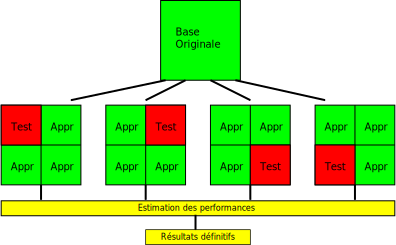
\includegraphics[width=15cm]{images/crossValid}
 \caption{Réalisation d'une validation croisée à $n$ éléments (ici 4) : La base d'exemples d'origine est décomposée en $n$ parts égales. La mesure de performance se fait $n$ fois, avec à chaque fois un apprentissage sur $n-1$ éléments et un test sur l'élément restant. La mesure de performance est réalisée sur les résultats des $n$ tests.}
 \label{fig:crossValid}
\end{figure}


Pour choisir les meilleurs paramètres de classifieur, j'ai effectué une recherche exhaustive par grille avec les paramètres suivants :

\begin{description}
 \item [C :] de 1 à 10000 en 15 pas logarithmique
 \item [gamma :] de 0.0001 à 1 en 15 pas logarithmique
 \item [j :] de 1 à 4, soit de 8 à 32 caractéristiques
\end{description}

L'optimisation a été réalisée à l'aide du logiciel rapid-i~\cite{mierswa2006} pour chaque modalité. Les indicateurs de performance calculés par validation croisée sont les suivants : Sensibilité, Spécificité. Le triplet de paramètre retenu est celui qui maximise la sensibilité.

Nous avons représenté pour chaque modalité le nuage de point positionnant chaque triplet dans un espace à deux dimensions (``Sensibilité'', ``Spécificité''). Cela permet de vérifier que le critère choisit (maximisation de la sensibilité) ne se fait pas trop au détriment de la spécificité.

De ce nuage de point nous pouvons voir le front de pareto. Ce type de diagramme permet de rechercher un optimum selon plusieurs critères incompatibles. Dans notre cas, nous voulons à la fois une sensibilité et une spécificité importante, sachant qu'il n'existe pas de jeu de paramètres ''parfaits`` qui permettent d'avoir 100\% aux deux. Dans notre cas, le front de pareto va permettre de vérifier que le choix par maximisation de la sensibilité ne se fait pas au détriment de la spécificité.


\subsubsection{Mesure de performance de la base d'apprentissage}

La mesure de performance décrite ici permet de sélectionner les meilleurs paramètres de génération de la base d'apprentissage, mais aussi une fois ces paramètres sélectionnés, de comparer les différentes techniques de correction du mouvement respiratoire. La recherche des meilleurs paramètres de la base d'apprentissage seront réalisés sur la base d'images Statiques afin de ne pas être influencé par les éventuels artefacts des autres modalités.

Pour un seuil donné, Le CAD va générer un ensemble d'agrégats associés à un score, comme présenté en \ref{lab:aggregatsCAD}. Il est ensuite possible d'évaluer la performance de ce CAD à l'aide de courbes F-ROC décrites en \ref{lab:FROC} en connaissant la vérité terrain.

Le seuil sélectionné pour générer les agrégats sera celui qui va maximiser la LLF (Fraction de Localisation de Lésion), c'est à dire celui qui va permettre de détecter un maximum de lésions. 

Cette sélection est réalisée selon l'algorithme suivant :

\begin{itemize}
 \item \emph{Sensibilité} := []
 \item Pour chaque seuil \emph{s} entre -2 et +2 (40 pas), faire :
 \item \hspace{1cm}\emph{CarteSeuillée} := Seuiller \emph{carte de Score} au seuil \emph{s}
 \item \hspace{1cm}\emph{Agrégats} := Calcul des agrégats de \emph{CarteSeuillée} (Score, classe, étendue).
 \item \hspace{1cm}Sensibilité[s] := Calcul Sensibilité(Agrégats)
 \item fin faire
 \item \emph{Seuil Optimal} := Seuil qui maximise la Sensibilité
\end{itemize}

Ce critère de sélection va naturellement engendrer un grand nombre de faux positifs, mais il faut garder à l'esprit qu'il sera utilisé pour réaliser des courbes F-ROC, qui indiquent une spécificité pour chaque nombre de faux positif en jouant sur un second seuil, toujours supérieur à celui retenu pour extraire les agrégats.

Le second critère utilisé pour pour comparer les bases d'apprentissage est la figure de mérite décrite en \ref{lab:AFROC}. Elle va comparer les scores des faux positifs de plus fort score pour chaque image avec les score  des vrais positifs de l'image.


\chapter{Analyse des résultats}

Dans ce chapitre je vais détailler les résultats obtenus par les méthodes présentées précédemment. Je commencerais par présenter les courbes obtenues lors de l'étape d'optimisation et d'adaptation du CAD aux données, puis je parlerais des résultats obtenus par ce CAD pour les différentes modalités.

\section{Optimisation des paramètres}

\begin{figure}[h!]
\begin{center}
 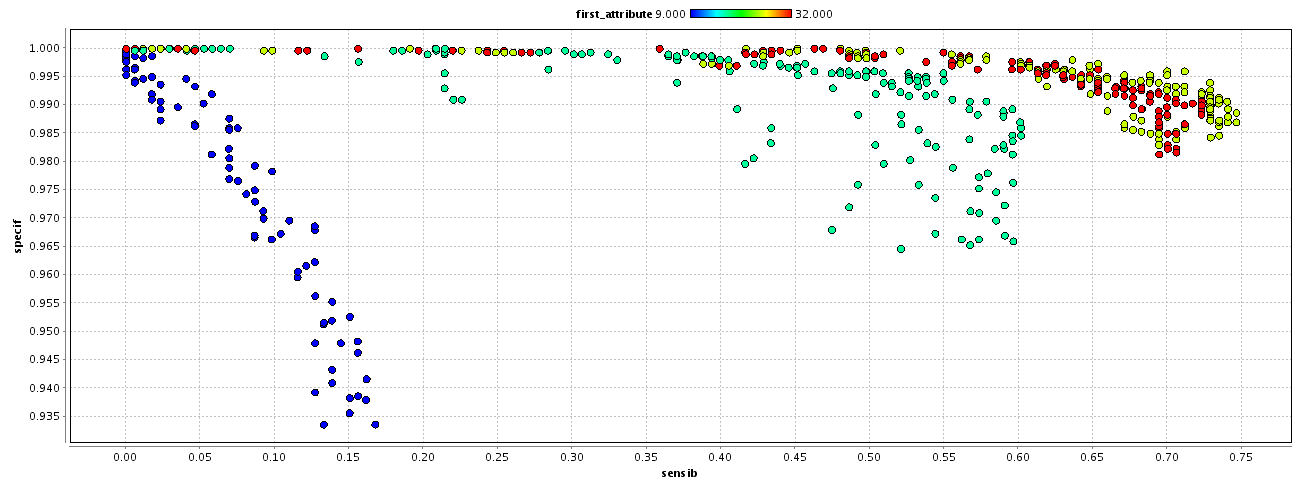
\includegraphics[width=14cm]{images/pareto_param_200.png}

{\small a) Base Témoin}
\vspace{0.5cm}

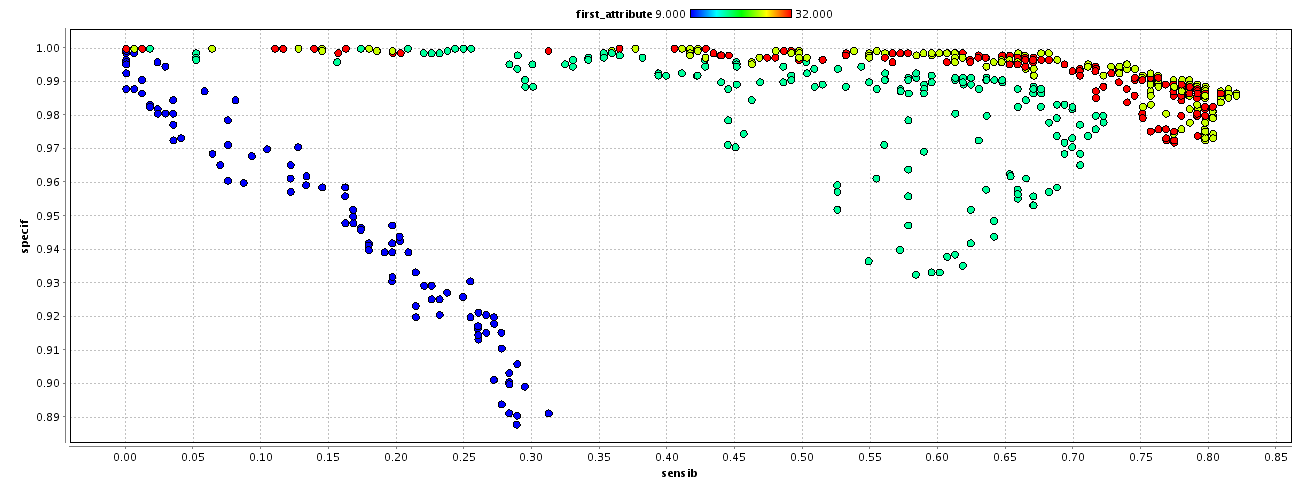
\includegraphics[width=14cm]{images/pareto_param_100.png}

{\small b) Base appauvrie}

 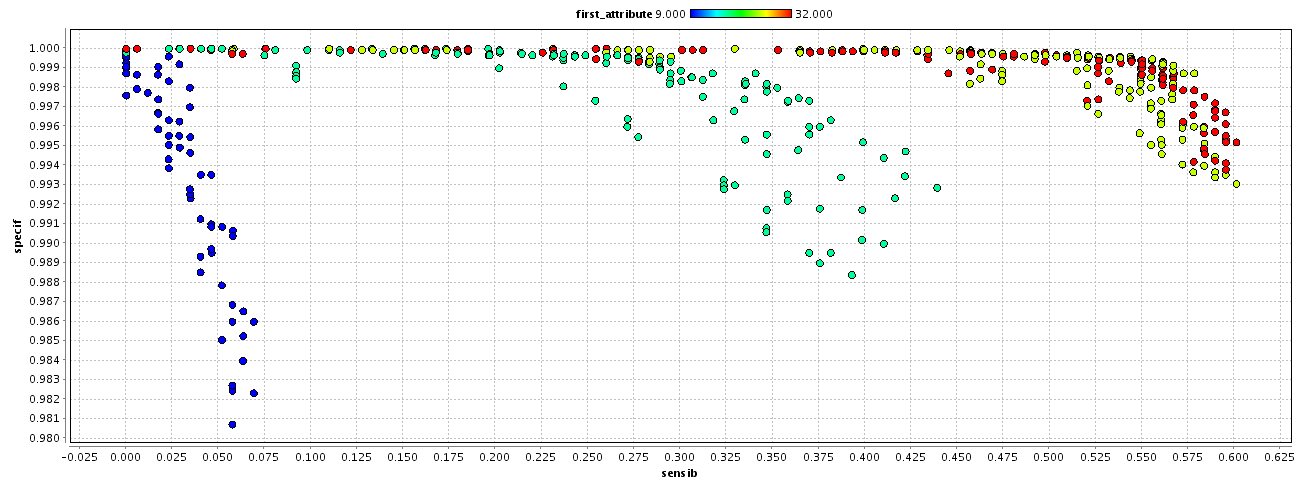
\includegraphics[width=14cm]{images/pareto_param_1000.png}
 
{\small c) Base enrichie}

\end{center}
 \caption{Fronts de pareto des résultats de la recherche des meilleurs paramètres du classifieur (1/2). Pour chaque triplet de paramètres (C, $\gamma$, j), la sensibilité et la spécificité sont reportées sur le graphique. Le code couleur correspond à la valeur de j. En a), la base témoin, avec 200 points négatifs par image et une normalisation \emph{moyenne}, en b) la base appauvrie avec 100 points négatifs par image et une normalisation \emph{moyenne}, et en c) la base enrichie avec 1000 points négatifs par image et une normalisation \emph{moyenne}.}
\label{fig:paretoParams1}
\end{figure}



\begin{figure}[h!]
\begin{center}


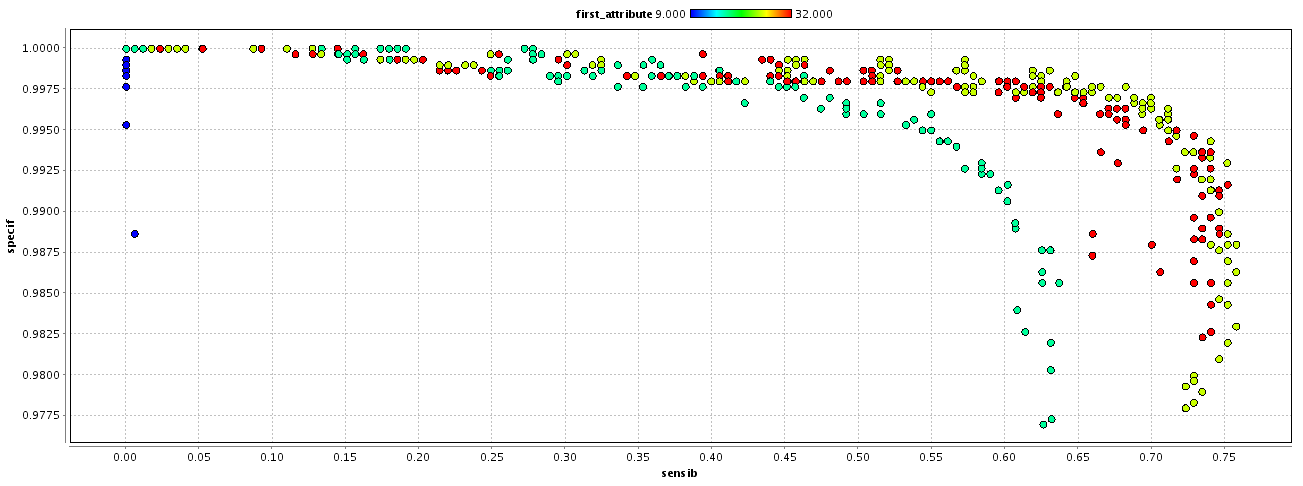
\includegraphics[width=14cm]{images/pareto_param_range.png}

{\small a) Base Normalisée -1/+1}

\vspace{0.5cm}

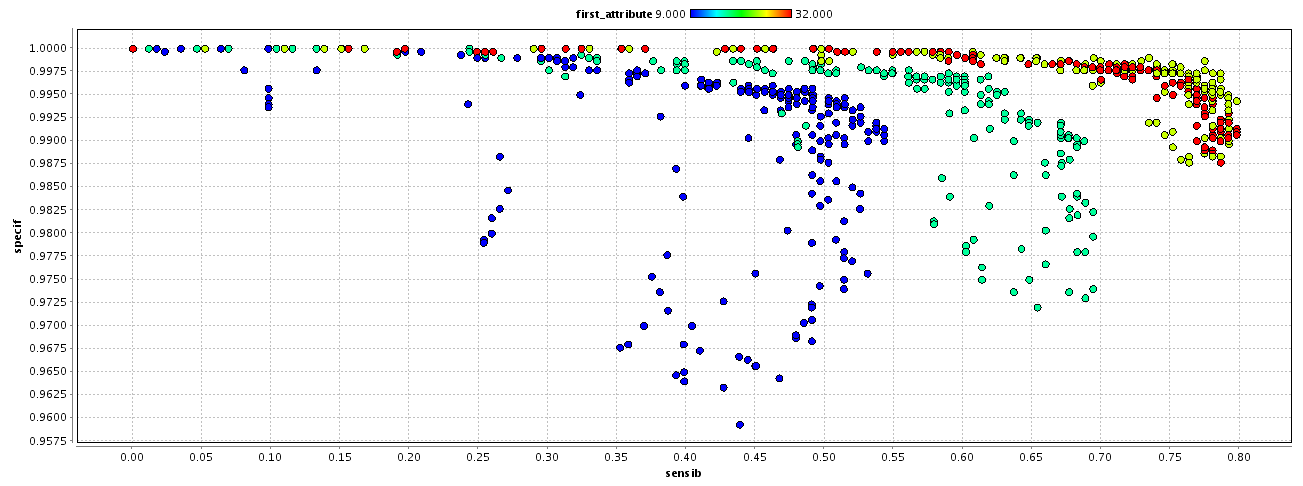
\includegraphics[width=14cm]{images/pareto_param_erosion.png}

{\small b) Base Érodée}

 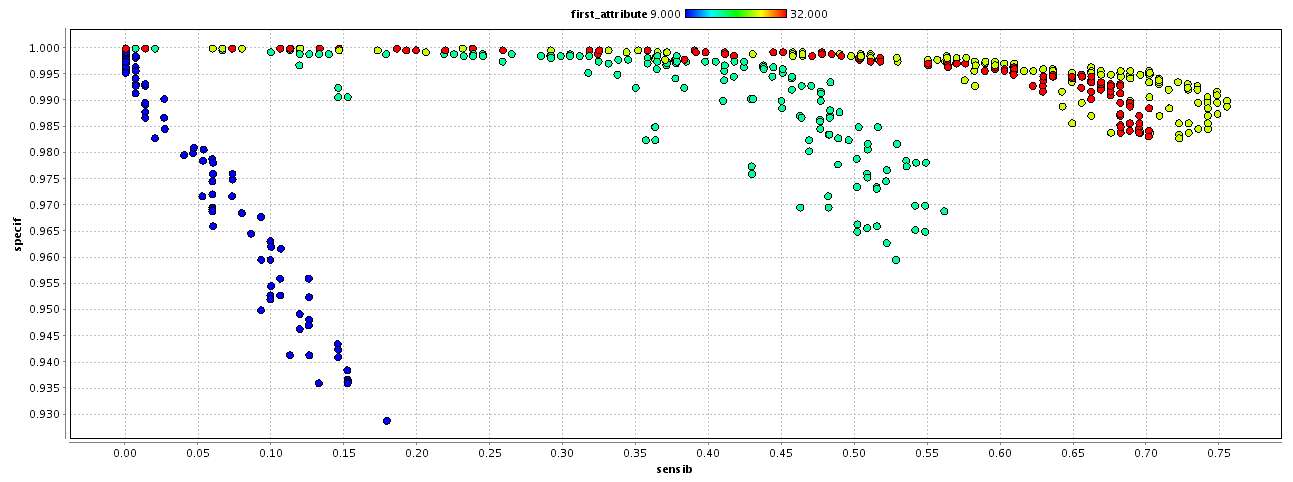
\includegraphics[width=14cm]{images/pareto_param_200_2.png}

{\small c) Base Témoin 2}

\end{center}
 \caption{Fronts de pareto des résultats de la recherche des meilleurs paramètres du classifieur (2/2). Pour chaque triplet de paramètres (C, $\gamma$, j), la sensibilité et la spécificité sont reportées sur le graphique. Le code couleur correspond à la valeur de j. En a) la base normalisation avec 200 points négatifs par image et une normalisation +1/-1. En b), la base érodée, avec 200 points négatifs par image et une normalisation \emph{moyenne}, en c) la base Témoin 2, réalisée de la même manière que la base témoin mais en retirant une image.. }
\label{fig:paretoParams2}
\end{figure}






Nous avons réalisé des mesures de performances pour 5 jeux de paramètres différents présentés ci-après. Les paramètres en \emph{italique} correspondent à ceux utilisés pour la base témoin.


\begin{itemize}
 \item Nombre de points de la base d'apprentissage (100, \emph{200}, 1000)
 \item Normalisation des données (\emph{moyenne}, +1/-1)
 \item Position des points de la base d'apprentissage (\emph{organe}, Érosion)
\end{itemize}


\begin{description}
 \item[Témoin : ] contient des données normalisées par la méthode moyenne avec 200 points extraits de chaque organe.
 \item[Érosion : ] contient des données normalisées par la méthode moyenne avec 200 points extraits de chaque organe érodée. C'est la seule base pour laquelle nous n'avons pas utilisé l'ensemble de l'organe hors tumeurs pour l'extraction des points.
 \item[Appauvrie : ] contient des données normalisées par la méthode moyenne avec 100 points extraits de chaque organe.
 \item[Enrichie : ] contient des données normalisées par la méthode moyenne avec 1000 points extraits de chaque organe.
 \item[Normalisation : ] contient des données normalisées par la méthode +1/1 avec 200 points extraits de chaque organe.
\end{description}

Pour vérifier que les paramètres du classifieur sont stables, une nouvelle base Témoin (Témoin 2) a été générée avec les données de seulement 14 images sur les 15 que nous avons simulé. Les points ''normaux`` ne sont pas non plus extraits aux mêmes endroits que pour la base Témoin. Nous allons donc vérifier que les paramètres optimaux du CAD ne sont pas dépendant de la base mais de ses paramètres.


\subsection{Sélection des meilleurs paramètres du classifieur}

Les paramètres du classifieur sont déterminés par une recherche par grille. Elle consiste à rechercher l'optimum en évaluant la performance ce chaque jeu de paramètre dans un ensemble déterminé à l'avance pour représenter . La performance de chaque triplet (C, $\gamma$, j) est estimée en réalisant une cross-validation à 5 validations sur l'ensemble de la base d'apprentissage.


Les paramètres sont choisis à partir du front de pareto figures \ref{fig:paretoParams1} et \ref{fig:paretoParams2} en maximisant la sensibilité.

Dans l'ensemble, on peut voir clairement que les points correspondant au premier niveau de décomposition (bleu foncé) ont une performance systématiquement inférieure aux autres. Pour la base témoin, la performance maximal est atteinte pour environ 15\% de sensibilité et une spécificité de 93.5\%, ce qui correspond à la valeur de spécificité la plus faible de tous les points de la base témoin. On observe cependant un front de pareto marqué, bien qu'en fort retrait par rapport aux autres niveaux de décomposition. Ce même constat se retrouve pour les bases appauvries et enrichies.

Les deux autres bases ont des comportements différents. Pour la base normalisée, les performances s'effondrent suffisamment pour que le classifieur soit quasiment incapable de discerner les classes, avec une sensibilité maximale de 1\% environ. Cela indique qu'il ne parvient pas à trouver une surface de séparation des données avec les paramètres indiqués. Puisque la normalisation moyenne parvient à mieux séparer les données pour ce niveau de décomposition, il est probable que la normalisation ne parvienne pas à homogénéiser les différentes dimensions de manière satisfaisante. Dans le cas de la base érodée, la simplification du problème de classification fait que les performances sont nettement en hausse avec des performances de l'ordre de 55\% de sensibilité pour 99.2\% de spécificité, ce qui est le score le plus élevé de toutes les bases.

Les performances du second niveau de décomposition (bleu ciel) sont toujours situées environ au barycentre entre les performances du premier niveau et celles des niveaux 3 et 4.

Les performances des décomposition de niveaux 3 (vert) et 4 (rouge) sont systématiquement meilleures que les autres mais sont entremêlées. La base Témoin et la base Appauvrie montrent une claire avance tant en terme de sensibilité que de spécificité pour 3 niveaux de décomposition. La base érodée ne montre quand à elle aucune différence de spécificité entre ces deux niveaux de décomposition, mais montre cependant une faible amélioration de la sensibilité pour les 4 niveaux (de 0.5\%). Quand à la base normalisée, on n'observe pas de réelles différences entre les deux niveaux de décomposition.

La table \ref{fig:paramsParams} référence tous les paramètres sélectionnés à partir des courbes de pareto. On peut observer que la sensibilité la plus importante est atteinte pour la base appauvrie, avec 82\% de bonne détection. Ce taux est sensiblement le même que celui de la base Érosion (80\%). Ces valeurs importantes par rapport aux autres peuvent s'expliquer par le fait que ces deux bases proposent un problème simplifié. Dans le cas de la base Érosion, les cas litigieux (discontinuités proches des bords des organes) ont été retirés de la base, ce qui simplifie le problème, tandis que pour la base appauvrie, c'est le nombre de points ''sain`` plus faible de la base d'apprentissage (1500 contre 3000) qui permet de rendre le problème plus simple à traiter au détriment de la généralisation du résultat trouvé aux images complètes.

Il est intéressant de constater que les performances en sensibilité pour les bases Appauvrie, Témoin et Enrichie sont inversement proportionnels à la taille de la base. En effet, plus la complexité de la base est importante, plus il devient difficile de trouver une surface de séparation efficace. Cependant, une base trop simpliste va engendrer une solution qui sera sans rapport avec la réalité, comme nous le verrons plus tard avec les courbes F-ROC.

Les valeurs de spécificité sont toutes très supérieures à 99\%, ce qui montre que le classifieur n'a pas de problèmes pour classer correctement les points sains. En effet, la base étant très déséquilibrée, avec un rapport de 17 points sains pour 1 point ''lésion`` dans la base témoin, il est normal il est normal que le classifieur favorise la classification des points ''sain''. Il existe des techniques permettant de compenser ce déséquilibre lors de l'apprentissage, mais tous les tests que nous avons réalisés n'ont pas montrés d'amélioration du résultat. En effet, l'étape de sélection du seuil (voir section suivante) permet de compenser ces différences.

Il est intéressant d'observer que les fronts de pareto de la base Témoin 2 sont très semblables à ceux de la base Témoin pour une décomposition au troisième niveau. Des disparités sont apparues Cela semble indiquer que la base est stable avec un nombre de points suffisant.

\begin{table}[h!]
	\begin{center}
		\begin{tabular}{c c c c c c}
  \hline
  a	& Base Témoin 	& Base Érosion	& Base appauvrie& Base enrichie & Base normalisée \\
  \hline
 C 	& 464		& 74		& 5412		& 5412		& 10000 \\
\hline
$\gamma$& 0.0053	& 0.0094	& 0.00031	& 0.0017	& 0.052 \\
\hline
j	& 3		& 3		& 3		& 4		& 3	\\
\hline
\hline
Sensibilité& 0.75	& 0.80		& \textbf{0.82}		& 0.60		& 0.76	\\
\hline
Spécificité& 0.99	& 0.99		& 0.99		& 0.99		& 0.99 \\
\hline
Précision& 0.98		& 0.98		& 0.97		& 0.99		& 0.98 \\
\hline
 		\end{tabular}

	\end{center}
\caption{Paramètres sélectionnés pour l'optimisation des performances sur les différentes bases. Sont indiqués pour chaque base le triplet de paramètres sélectionné ainsi que sa position sur le front de pareto.}
\label{fig:paramsParams}
\end{table}

\FloatBarrier

\subsection{Courbe Free-ROC}

Les courbes Free-ROC de la figure \ref{lab:froc_comp_static} permettent de comparer les performances du CAD sur les différentes bases d'apprentissage. Les courbes ont volontairement été tronquées à 40 faux positifs par image, car ce nombre est déjà trop important pour un système CAD.

On peut observer que les courbes correspondants aux bases Témoin et Enrichie atteignent leur maximum de performances pour un nombre de faux positifs relativement faible par rapport aux autres bases : entre 17 et 20 faux positifs pour ces bases, contre plus de 40 pour les bases Appauvrie et Érosion. Cela tends à montrer que le système CAD est plus performant pour ces bases car il crée moins d'agrégats là ou il n'y a pas de lésions.

En ce qui concerne la sensibilité maximale obtenue sur les courbes, elle est atteinte pour la base témoin avec environ 62\% de sensibilité, suivie par la base appauvrie avec 60\%, mais pour un nombre de faux positifs beaucoup plus important (38 contre 18 pour la base Témoin). La troisième courbe est la courbe Normalisation, suivie par la base enrichie puis la base Érosion. Il est important de noter que les sensibilités maximales observées sont très proches, entre 55\% et 62\%, ce qui indique que la qualité de la base d'apprentissage n'a pas d'impact réel sur la sensibilité maximale atteinte par le CAD, mais qu'il pourra être plus ou moins difficile pour ce dernier de différencier les lésions du bruit de fond. 

En pratique, on choisira le seuil pour avoir la certitude d'avoir un nombre de faux positifs ``raisonnable'' par image. Dans notre cas, les images contiennent environ 10 lésions par image. Il peut être intéressant de comparer les performances des bases pour ratio de 1 faux positif par lésion, soit pour 10 faux positifs. Dans ce cas, la base Témoin est au coude à coude avec la base Enrichie, à environ 55\%, ce qui est déjà très proche de leur performances maximales. La base Normalisation et la base Appauvrie sont quand à elles à 40\% de sensibilité, tandis que la base Érosion atteint 35\%.


\begin{figure}[h!]
 
 \begin{center}
   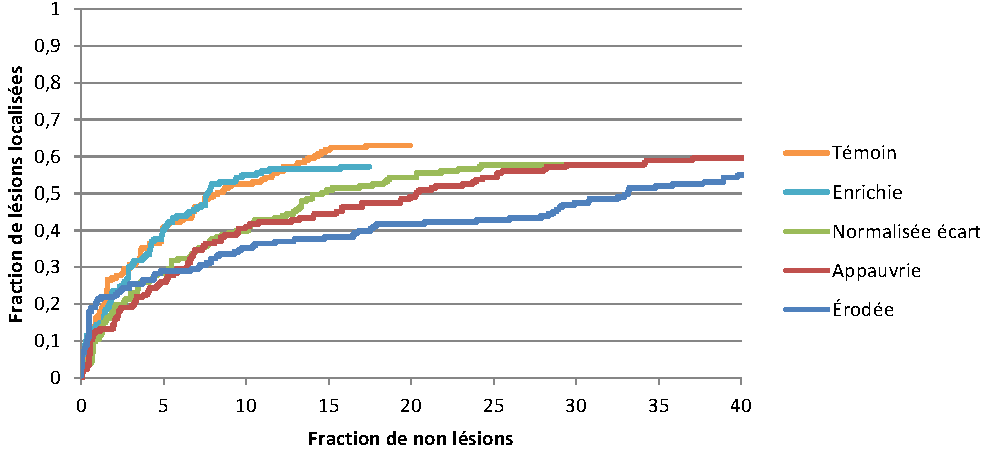
\includegraphics[width=15cm]{images/FROC_param}
 \end{center}
 \caption{Courbe Free-ROC comparant les performances du CAD sur une base témoin (normalisation \emph{moyenne} et 200 points négatifs par image), sur une base enrichie (1000 points négatifs par image), sur une base appauvrie (100 points négatifs par image), sur une base normalisée différemment (normalisation entre -1 et +1 et 200 points négatifs par image) et enfin sur une base de 100 points négatifs par image mais dont les volumes ont été érodés de 2 voxels.}
 \label{lab:froc_comp_static}
\end{figure}


\subsection{Comparaison des performances JAFROC}

La comparaison des performances obtenues par l'algorithme JAFROC \cite{chakraborty1990free} de la figure \ref{lab:fom_param} nous montre les FDM (Figure de Mérite) obtenues pour les différentes bases. Les FDM des bases Témoin, Érosion et Enrichie sont quasiment au même niveau à 0.18, mais les barres d'erreurs semblent montrer un léger avantage pour la base Témoin.

Les bases Normalisation et Appauvrie quand à elles ont une FDM de 0.1 environ, ce qui indique une performance plus faible que les autres.

D'un point de vue statistique, La p-value fournie par le logiciel est de 0.049, ce qui ne permet pas de pouvoir annoncer avec une fiabilité de 95\% que le test est significatif, c-à-d que les FDM sont effectivement toutes différentes. Cela se vérifie aisément en regardant l'étendue des barres d'erreur. Mais il faut noter que cette FDM est basée sur une méthode avec une puissance statistique faible, ce qui signifie qu'elle sous-estime la p-value.

\begin{figure}[h!]
 \begin{center}
   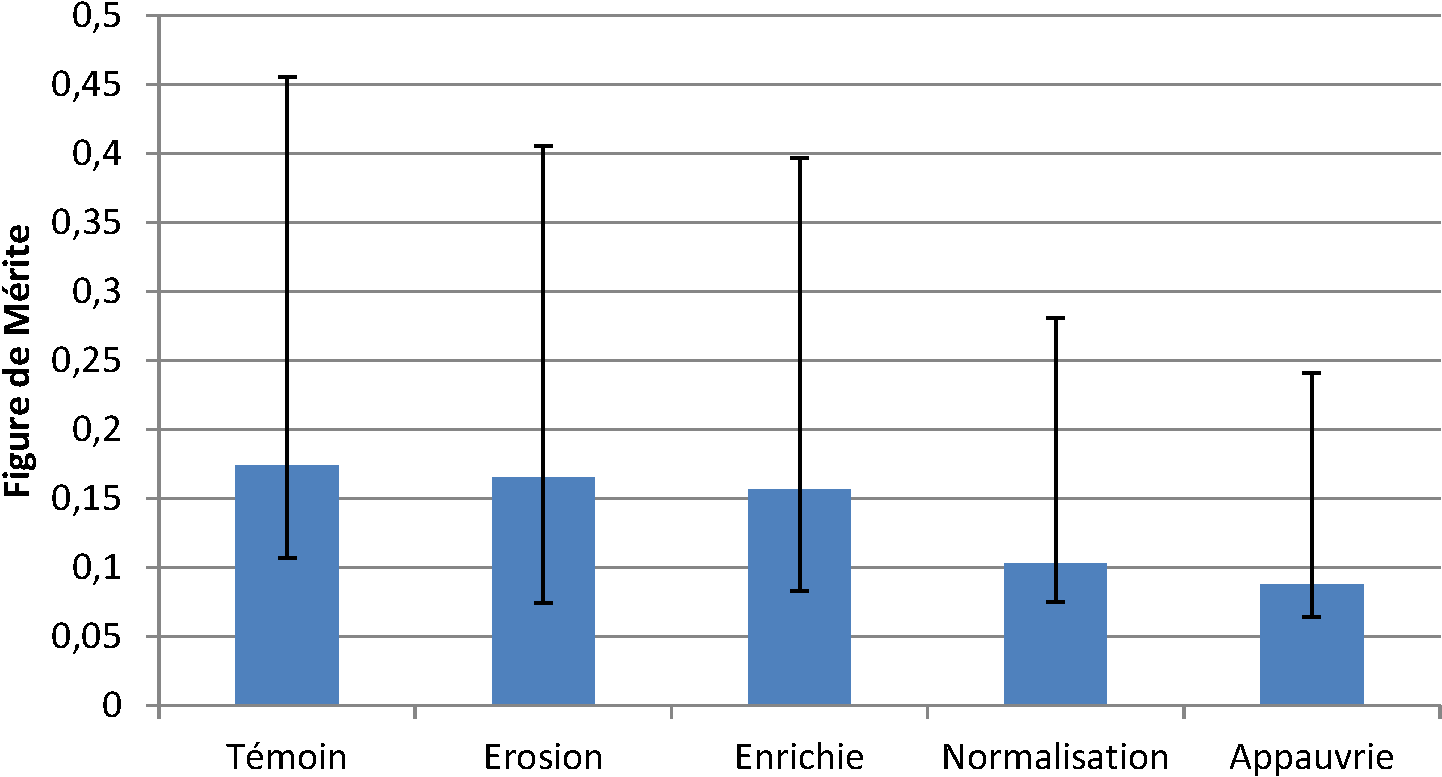
\includegraphics[width=15cm]{images/FOM_param}
 \end{center}
 \caption{Les FOM (Figure de Mérite) obtenues pour les différents paramètres}
 \label{lab:fom_param}
\end{figure}

\subsection{Conclusion}

Nous avons vu que tous les indicateurs indiquent que le maximum de performance est apporté apr la base Témoin. De plus, les  performances relativement proches de la seconde base semblent indiquer que le performances sont stables. Nous allons donc conserver les paramètres de cette base pour les comparaison futures entre les modalités :

Pas d'érosion, une normalisation visant à ramener la moyenne et l'écart-type sur les caractéristiques à 1, et 200 points extraits de chaque images de la base d'apprentissage.
 

\FloatBarrier

\section{Comparaison des performances des différentes méthodes sur le Poumon}

Les paramètres de génération de la base d'apprentissage retenus sont ceux de la base Témoin. Ils correspondent aux choix suivants :

\begin{itemize}
 \item 200 points tirés aléatoirement dans le volume complet du poumon de chaque image (hors tumeurs)
 \item normalisation par neutralisation de la moyenne et de la variance , tels que $\mu, \sigma) = (1,1)$
\end{itemize}


Quatre modalités seront comparées. ET-Static correspond aux images de la ``vérité terrain'', à savoir des images sans mouvement respiratoire. Elle doit donner la performance haute. ET-NoCorr à l'inverse correspond aux images simulées avec mouvement respiratoire mais reconstruites sans aucune correction de mouvement. Elle représente la marge basse. ET-IM corresponde aux images reconstruites avec la correction de mouvement post-reconstruction, et ET-LOR aux images reconstruites avec correction de mouvement pendant la reconstruction.


\begin{figure}[h!]

\begin{center}
 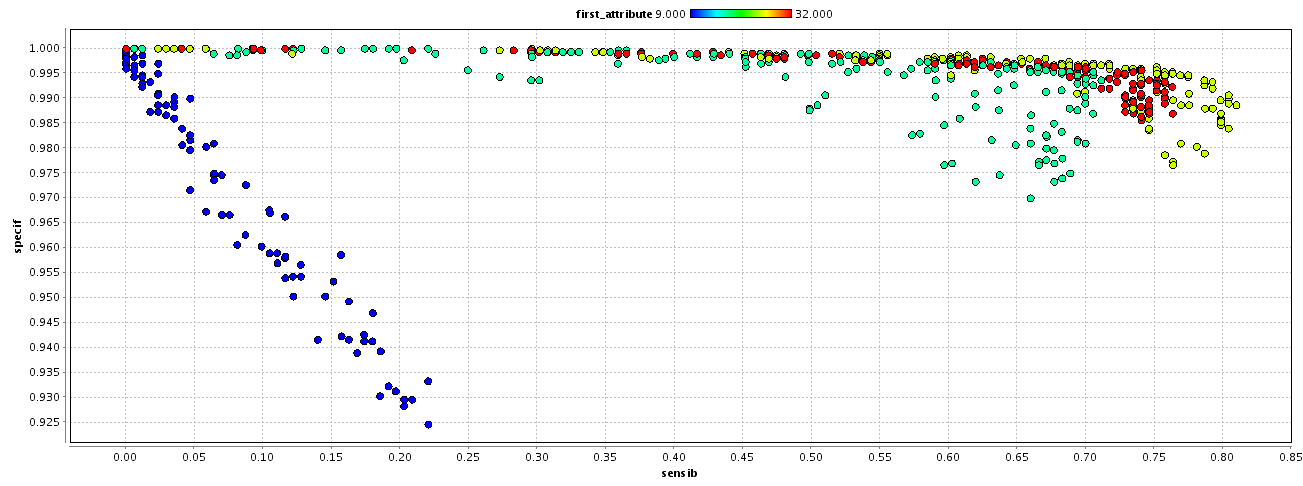
\includegraphics[width=14cm]{images/pareto_mod_IM.png}

{\small a) ET-IM}
\vspace{0.5cm}

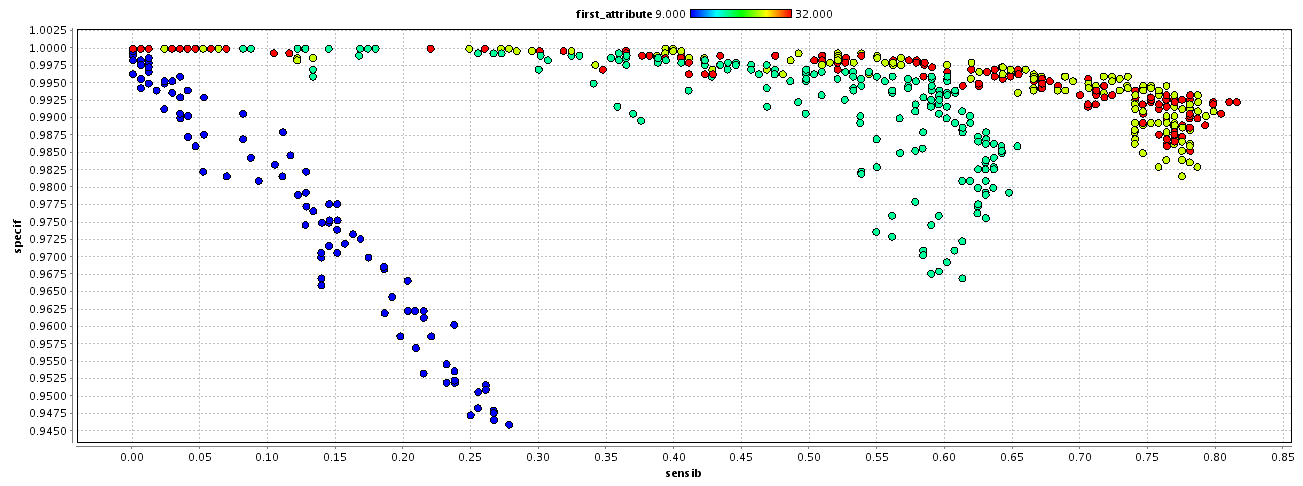
\includegraphics[width=14cm]{images/pareto_mod_LOR.png}
 
{\small b) ET-LOR}
\vspace{0.5cm}

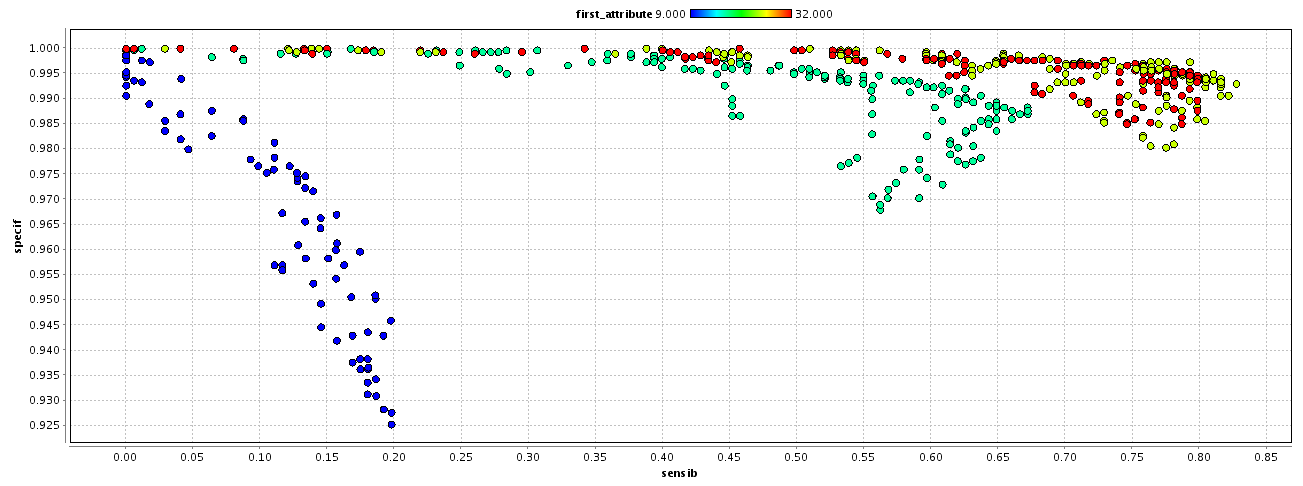
\includegraphics[width=14cm]{images/pareto_mod_NoCorr.png}

{\small c) ET-NoCorr}

\end{center}
 \caption{Fronts de pareto des résultats de la recherche des meilleurs paramètres du classifieur pour les différentes modalités, avec 200 points négatifs par image. Pour chaque triplet de paramètres (C, $\gamma$, j), la sensibilité et la spécificité sont reportées sur le graphique. Le code couleur correspond à la valeur de j. a) représente la correction d'image ET-IM, b) les images non corrigées du mouvement, et c) les images corrigées par la méthode LOR.}
\label{fig:paretoModalite} 
\end{figure}








\begin{table}[h!]
	\begin{center}
		\begin{tabular}{c| c c c c c}
  \hline
  a	& Base Statique	& Base IM	& Base LOR	& Base NoCorr	\\
  \hline
 C 	& 464		& 10000		& 10000		& 10000		\\
\hline
$\gamma$& 0.0053	& 0.00097	& 0.00031	& 0.00055	\\
\hline
j	& 3		& 3		& 4		& 3		\\
\hline
\hline
Sensibilité& 0.75	& 0.81		& 0.82		& 0.83	\\
\hline
Spécificité& 0.99	& 0.99		& 0.99		& 0.99		\\
\hline
Précision& 0.98		& 0.98		& 0.98		& 0.98		\\
\hline
 		\end{tabular}

	\end{center}
\caption{Paramètres sélectionnés pour l'optimisation des performances du Poumon. Sont indiqués pour chaque base le triplet de paramètres sélectionné ainsi que sa position sur le front de pareto.}
\label{fig:paramsModPoumon}
\end{table}

\subsection{Sélection des meilleurs paramètres du classifieur}

De la même manière que pour la sélection de la méthode de génération de la base d'apprentissage, il faut adapter les paramètres du classifieur aux différentes bases d'apprentissage.

La figure \ref{fig:paretoModalite} montre les nuages de points associés aux différents triplets de paramètres (C, $\gamma$, $j$) pour chaque modalité. La référence sera toujours la base Témoin de la figure \ref{fig:paretoParams1}.a, car elle correspond à la vérité terrain.

%%%%%%%%% ?????????????? %%%%%%%%%%%%%
Il est étonnant de constater que la base \ref{fig:paretoParams1}.a, qui correspond à la modalité statique, offre les plus mauvaises performances pour la décomposition de niveau 1 (17\% de sensibilité) de toutes les modalités. La mauvaise performance de cette base d'apprentissage se retrouve pour tous les niveaux de décomposition. A l'inverse, Les nuages de points des autres modalités ont la même répartition que ceux de la base Statique, par opposition aux distributions des bases érodées ou normalisées vues dans la partie précédente. 

On peut observer qu'il y a une forte corrélation entre la sensibilité et la spécificité des points pour toutes les modalités au premier niveau de décomposition.

La modalité ayant les meilleures performances pour la décomposition de niveau 2 est ET-IM, avec plus de 70\% de sensibilité, comparés aux 60\% de la base Statique. 

Les meilleures performances du CAD sont atteintes pour le troisième niveau de décomposition pour toutes les modalités sauf ET-LOR, avec une sensibilité d'environ 81 à 84\% excepté pour ET-Static avec 75\%, confirmant la tendance observée au premier niveau de décomposition.

La spécificité observée pour les meilleurs jeux de paramètres est sensiblement la même quelque soit la modalité, entre 99\% et 99.5\%.

\subsection{Courbes Free-ROC}

Les courbes F-ROC obtenues sur les différentes modalités sont présentées dans la figure \ref{fig:froc_mod}. 

Toutes les courbes on une NLF (Nombre de faux positifs moyen par image) à peut près équivalente entre 20 et 24 , excepté ET-LOR avec une NLF de 34. Cependant, les performances en LLF (proportion des lésions localisées) de ET-LOR sont constantes à partir d'une NLF de 20 environ. 

L'ordre des courbes est constant pour tous les NLF à partir de 5 faux positifs par image. Au delà de cette limite, les performances des images statiques sont supérieures à celles de ET-IM de 1 à 5\%, tandis que ET-IM a des performances supérieures de 3 à 10\% à celles des images non Corrigées et de ET-LOR. Ces deux dernières modalités ont des performances quasiment identiques.

Cependant, en dessous de 5 faux positifs par image, les courbes sont trop proches pour pouvoir en déduire une tendance.


Dans sa globalité, le graphique montre que le maximum de performances est apporté par la base Statique, suivi par la base ET-IM. Les bases ET-LOR et Non corrigées sont très proches l'une de l'autre mais nettement en dessous des deux premières en terme de LLF à NLF égale.

\begin{figure}[h!]
 \begin{center}
   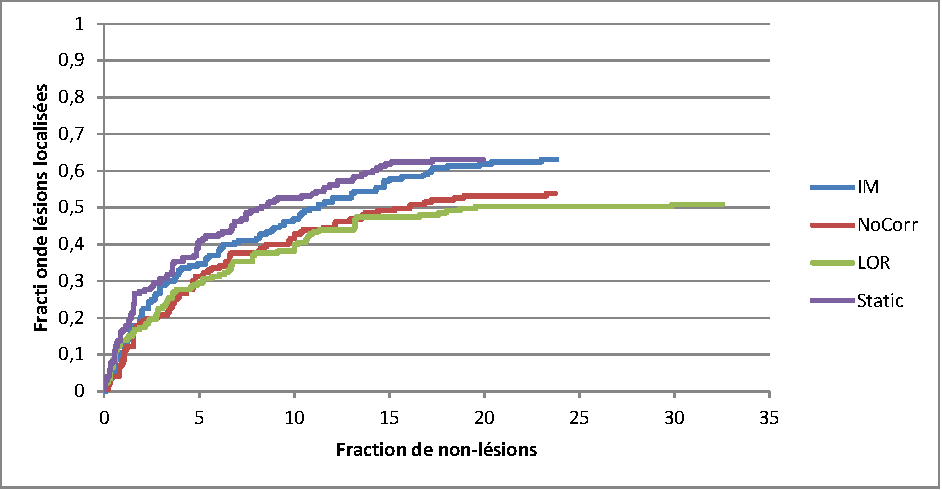
\includegraphics[width=13cm]{images/FROC_mod}
 \end{center}
 \caption{Courbe Free-ROC comparant les performances du CAD selon les modalités de correction du mouvement respiratoire.}
 \label{fig:froc_mod}
\end{figure}


\subsection{Comparaison des performances JAFROC}

Les Figures de mérite obtenues par l'algorithme de JAFROC sont présentées dans la figure \ref{fig:fom_mod}. Cependant, on observe une tendance proche de celle observée sur les courbes F-ROC pour la modalité Statique : Ces images sont en tête suivies par ET-IM. Il est intéressant de noter que les valeurs de ET-IM et ET-LOR sont relativement proches, y compris leurs mesures d'erreur, ce qui indique que l'algorithme JAFROC peine à les distinguer l'une de l'autre. ET-NoCorr est quand à lui nettement en retrait. 

\begin{figure}[h!]
 \begin{center}
   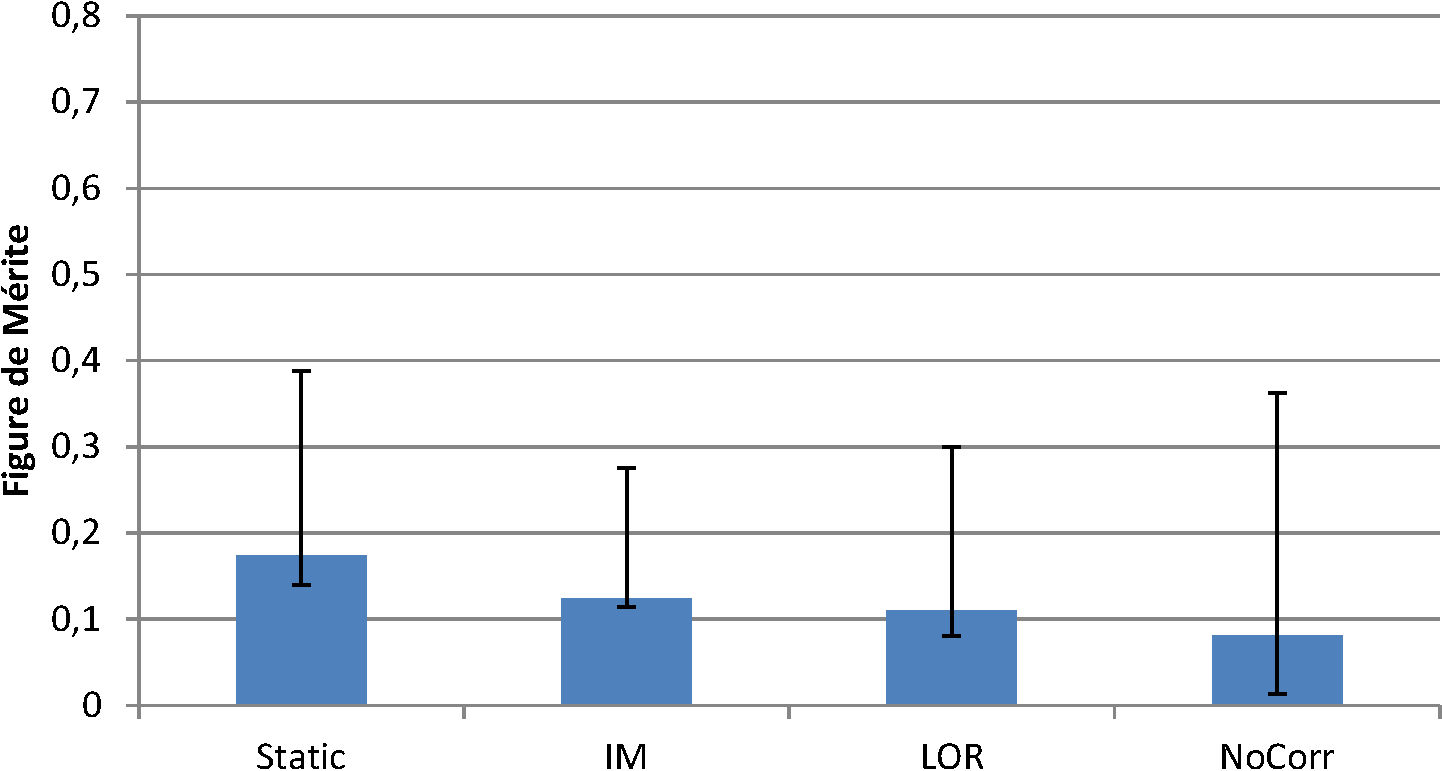
\includegraphics[width=13cm]{images/FOM_mod}
 \end{center}
 \caption{Les FDM (Figure de Mérite) obtenues pour les différentes modalités.}
 \label{fig:fom_mod}
\end{figure}

\subsection{Conclusion}

Les résultats présentés précédemment indiquent que les techniques de correction du mouvement respiratoire améliorent les performances en détection par rapport aux images non corrigées. Le résultat est net pour ET-IM, surtout lorsque l'on regarde les courbes F-ROC. Il est plus difficile de statuer sur ET-LOR, dont les performances selon JAFROC sont au même niveau que celles de ET-IM, mais qui est nettement moins performant que ce dernier sur les courbes F-ROC.


\FloatBarrier

\section{Comparaison des performances des différentes méthodes Foie}


\subsection{Sélection des meilleurs paramètres du classifieur}



Les différents graphiques nous montrent une répartition des performances très différente de celle observée précédemment pour les travaux sur la base Poumon. 

Pour le premier niveau de décomposition, ET-Static, ET-IM et ET-LOR montrent une très grande dispersion des valeurs de performances. ET-NoCorr par contre montre des points plus proches, mais avec des sensibilités très faibles (inférieures à 15\%). Cette dispersion montre une rupture par rapport à la corrélation observée sur les bases du foie.

De la même manière que sur les données ne contenant que le premier niveau de décomposition, les performances obtenues pour $j=2$ montrent une dispersion très importante des points de donnée pour ET-Static et ET-IM. Le nuage de points correspondant à ET-LOR est plus proche de ceux observés précédemment. ET-NoCorr est clairement en difficulté car l'apport des informations du second niveau de décomposition diminue les performances maximales du CAD en sensibilité.

En ajoutant les informations des niveaux de décomposition supérieurs, on observe une amélioration nette des performances, surtout pour ET-NoCorr. Toutes les modalités bénéficie des informations ajoutées par le 4è niveau de décomposition. Cela semble indiquer que le classifieur est moins adapté pour gérer ces données. 

 Comme pour la base Poumon, ET-IM est la modalité ayant la sensibilité la plus forte avec 68\% (voir tableau \ref{fig:paramsModFoie}). Et cette fois ci, ET-Statique est seconde avec 62\% , 

\begin{figure}[h!]

\begin{center}
 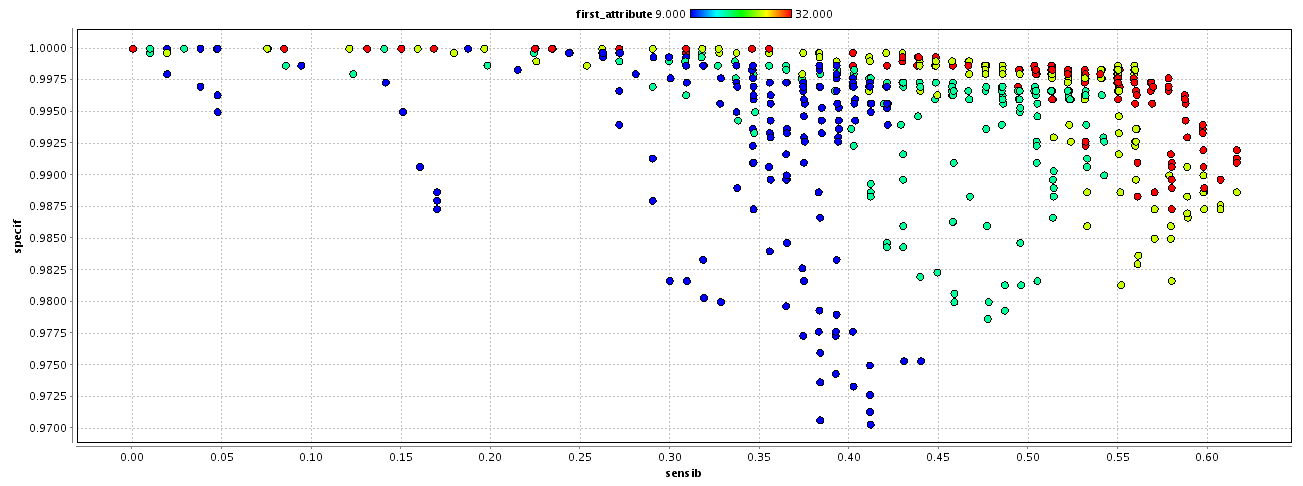
\includegraphics[width=14cm]{images/pareto_mod_Static19.png}

{\small a) ET-Static}
\vspace{0.5cm}

 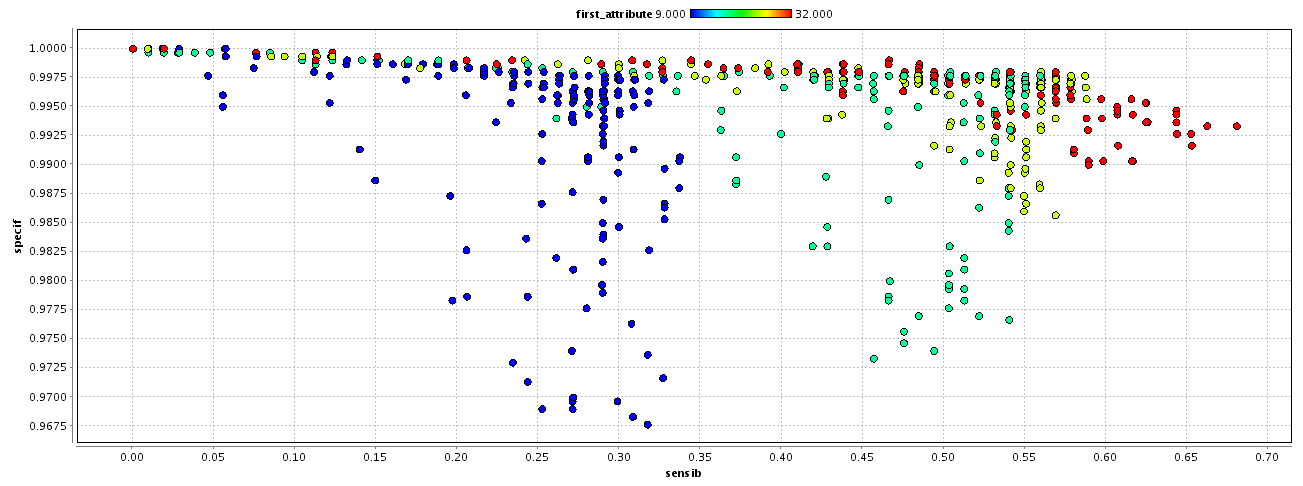
\includegraphics[width=14cm]{images/pareto_mod_IM19.png}

{\small b) ET-IM}

\end{center}
 \caption{Fronts de pareto des résultats de la recherche des meilleurs paramètres du classifieur pour les différentes modalités, avec 200 points négatifs par image. Pour chaque triplet de paramètres (C, $\gamma$, j), la sensibilité et la spécificité sont reportées sur le graphique. Le code couleur correspond à la valeur de j. a) représente la correction d'image ET-Static, b) les images corrigées du mouvement post-reconstruction.}
\label{fig:paretoModalite19_1}
\end{figure}

\begin{figure}[h!]

\begin{center}
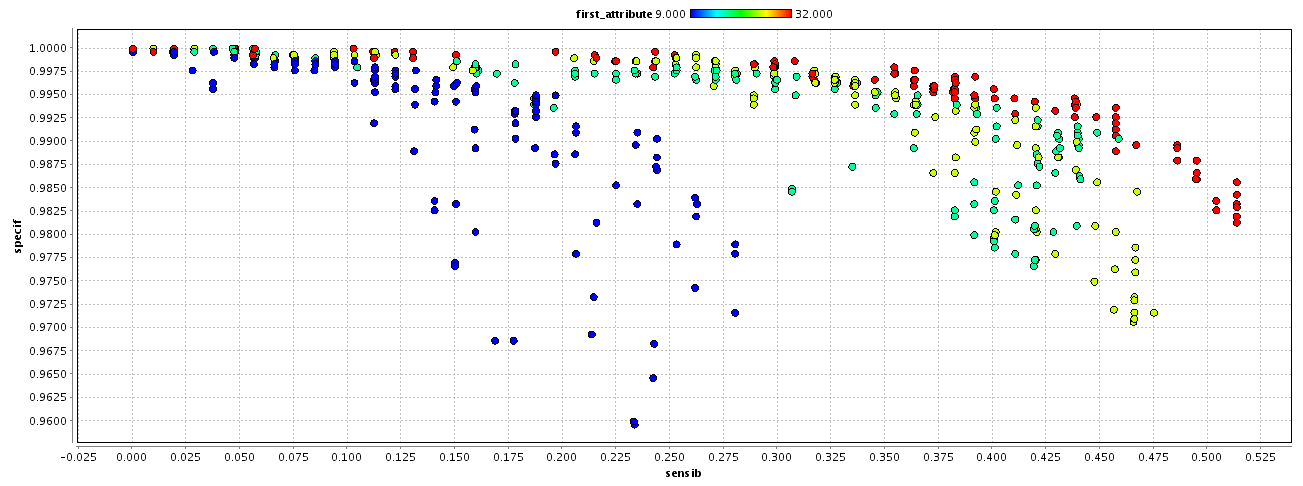
\includegraphics[width=14cm]{images/pareto_mod_LOR19.png}
 
{\small c) ET-LOR}
\vspace{0.5cm}

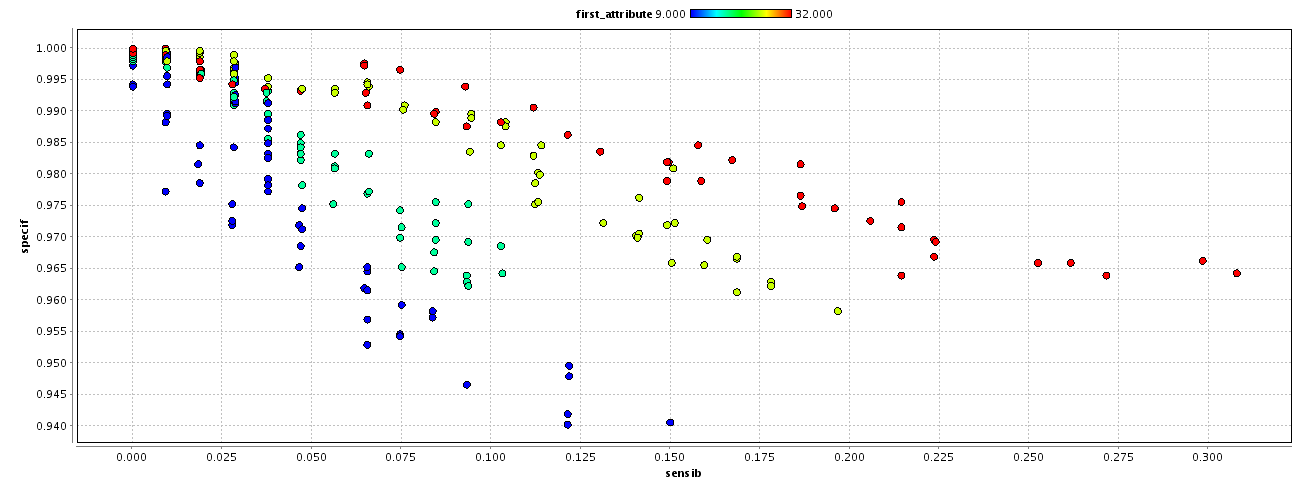
\includegraphics[width=14cm]{images/pareto_mod_NoCorr19.png}

{\small d) ET-NoCorr}

\end{center}
 \caption{Fronts de pareto des résultats de la recherche des meilleurs paramètres du classifieur pour les différentes modalités, avec 200 points négatifs par image. Pour chaque triplet de paramètres (C, $\gamma$, j), la sensibilité et la spécificité sont reportées sur le graphique. Le code couleur correspond à la valeur de j. c) représente la correction d'image pendant la reconstruction et d) le images non corrigées.}
\label{fig:paretoModalite19_2} 
\end{figure}

% Static : 857.6958985908936	0.001709975946676697	32.0	0.9790779315594078	0.6160173160173159	0.992
% LOR	 : 251.18864315095797	0.005323362023203629	32.0	0.969422309209811	0.5134199134199134	0.9856666666666667 
% NoCorr : 5411.6952654646375	0.001709975946676697	32.0	0.9417478291936561	0.30779220779220784	0.9643333333333333
% IM	 : 5411.6952654646375	5.49280271653059E-4	32.0	0.9826195691007659	0.6805194805194804	0.9933333333333334
\begin{table}[h!]
\begin{center}
		\begin{tabular}{c| c c c c c}
  \hline
  a	& Base Statique	& Base IM	& Base LOR	& Base NoCorr	\\
  \hline
 C 	& 858		& 5412		& 251		& 5412		\\
\hline
$\gamma$& 0.002		& 0.00055	& 0.0053	& 0.0017	\\
\hline
j	& 4		& 4		& 4		& 4		\\
\hline
\hline
Sensibilité& 0.62	& 0.68		& 0.51		& 0.31	\\
\hline
Spécificité& 0.99	& 0.99		& 0.99		& 0.96		\\
\hline
Précision& 0.98		& 0.98		& 0.97		& 0.94		\\
\hline
 		\end{tabular}

\end{center}
\caption{Paramètres sélectionnés pour l'optimisation des performances du CAD sur la base Foie. Sont indiqués pour chaque base le triplet de paramètres sélectionné ainsi que sa position sur le front de pareto.}
\label{fig:paramsModFoie}
\end{table}


\subsection{Comparaison des performances JAFROC}

\begin{figure}[h!]
 \begin{center}
   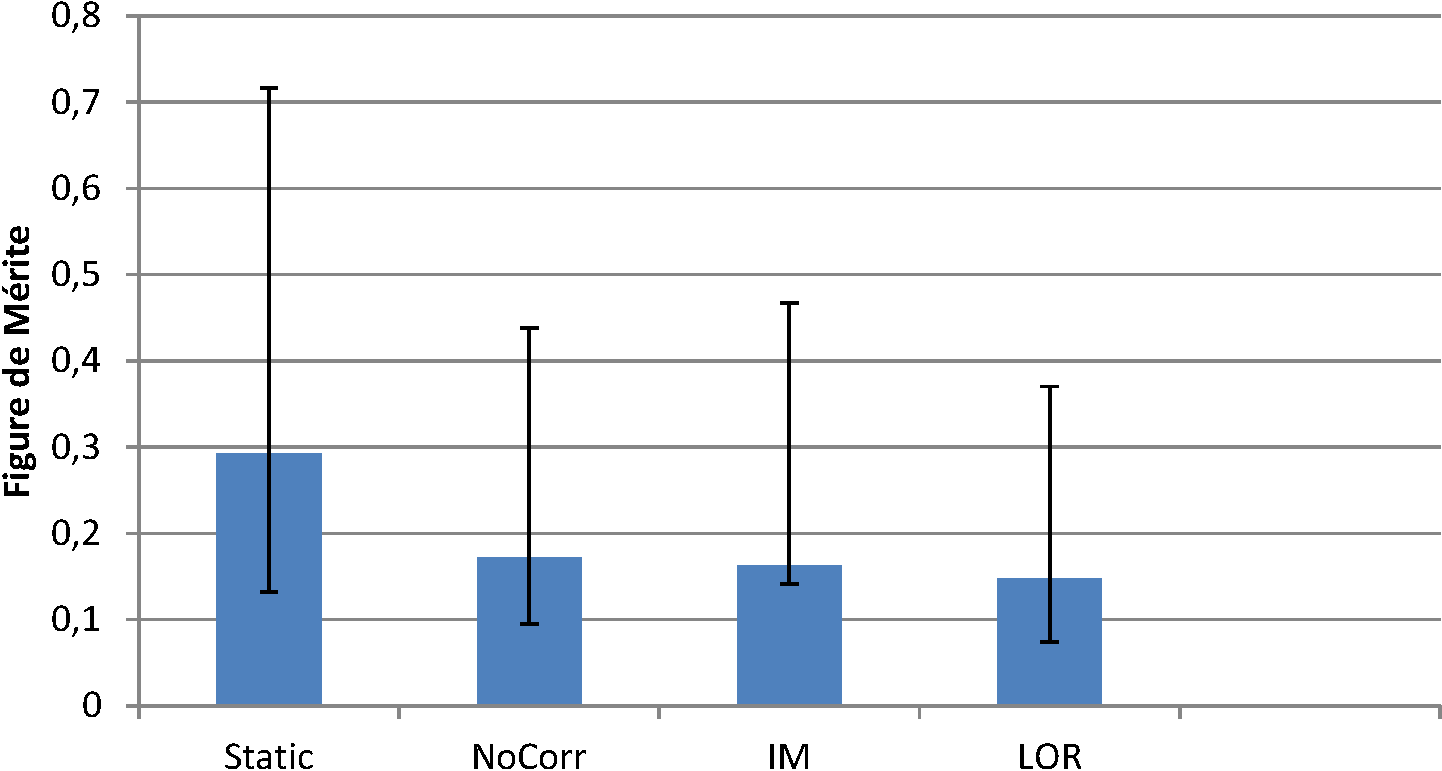
\includegraphics[width=15cm]{images/FOM_mod19}
 \end{center}
 \caption{Les FDM (Figure de Mérite) obtenues pour les différentes modalités.}
 \label{fig:fom_mod19} 
\end{figure}


Les Figures de mérite obtenues par l'algorithme de JAFROC sont présentées dans la figure \ref{fig:fom_mod19}. La p-value est de 0.1, ce qui ne permet pas de déclarer que statistiquement les données sont différentes : 
Il n'est pas étonnant de constater que les FOM sont plus élevées que précédemment car le nombre de faux positifs est pratiquement deux fois inférieur à celui obtenu pour le poumon, ce qui est le signe que le classifieur réussi mieux à discerner les vrai positifs.

On observe que les images statiques ont un score supérieur de 60\% environ à celui des images Non corrigées. Par contre, il est surprenant de constater que les deux techniques de correction du mouvement respiratoire ont un score égal ou plus faible que les images non corrigées, en contradiction avec les résultats de l'analyse F-ROC. Cependant, la proximité des valeurs ne permet pas de montrer une réelle hiérarchie entre les modalités. Tout au plus pourrait-on observer que l'étendue des barres d'erreur semble indiquer que ET-IM aurait de meilleures performances que les images non Corrigées, elles-mêmes supérieures aux images ET-LOR, mais il est n'est pas possible de se prononcer de manière définitive à partir de ces données. 



\subsection{Courbes Free-ROC}

\begin{figure}[h!]
 \begin{center}
   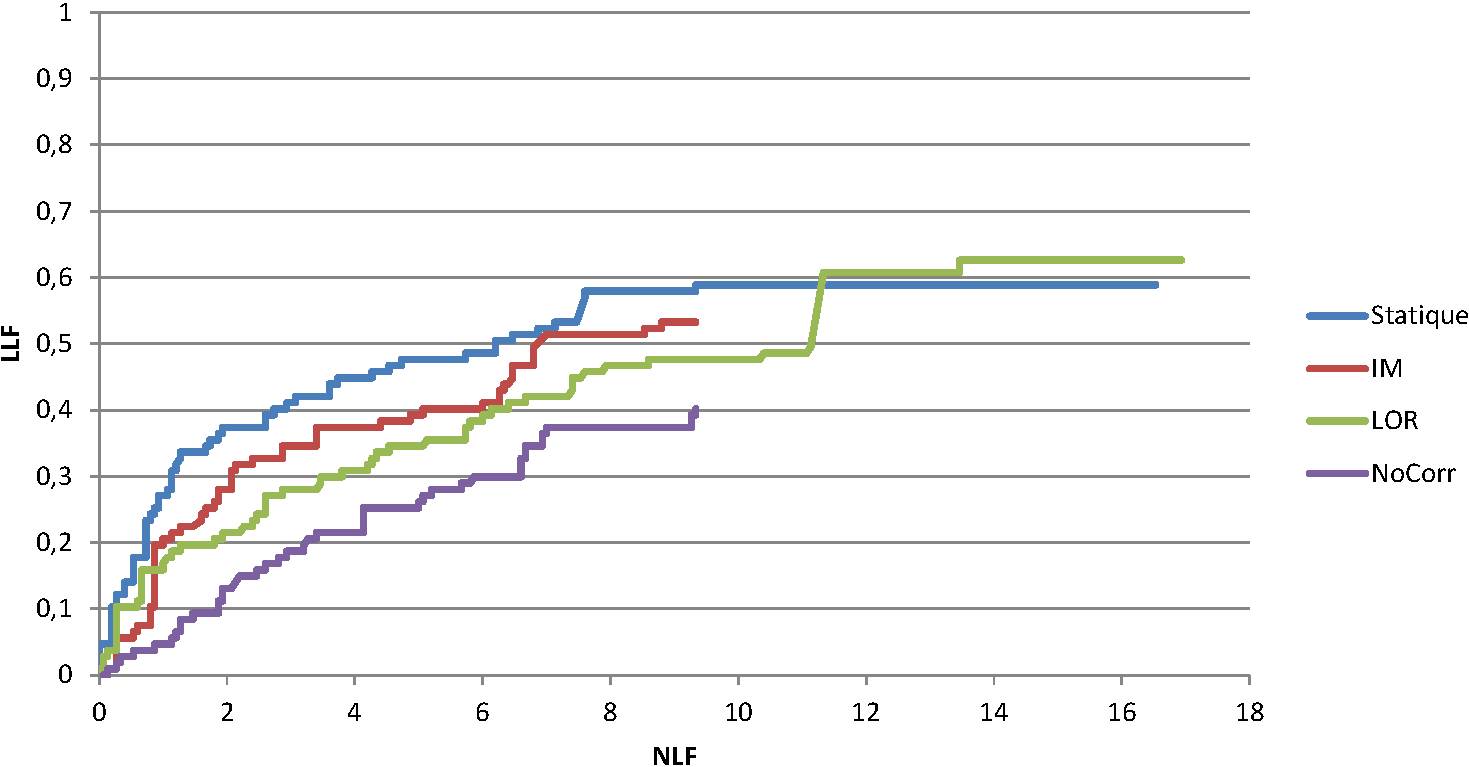
\includegraphics[width=15cm]{images/FROC_mod19}
   \vspace{-0.3cm}
 \end{center}
 \caption{Courbe Free-ROC comparant les performances du CAD selon les modalités de correction du mouvement respiratoire.}
\label{fig:froc_mod19}
\end{figure}


Les courbes Free-ROC de la figure \ref{fig:froc_mod19} montrent un ordre différent de celui présenté par l'analyse JAFROC.

Le maximum de performances est apporté par les images statiques, suivi par les images ET-IM, puis ET-LOR et enfin ET-NoCorr. Contrairement au poumon, les courbes sont relativement bien séparées avec une différence de sensibilité de 20\% entre les images non corrigées et statiques. 

Il est étonnant d'observer que les images statiques et ET-LOR ont tous les deux un NLF maximum d'environ 17, très supérieur à celui de ET-IM et des images non corrigées qui ne dépassent pas 9 faux positifs par image. Mais comme dans les cas précédents, ce nombre important de faux positifs n'apporte qu'une amélioration très faible de la sensibilité pour les images Statiques, au contraire de ET-LOR où un important bond de sensibilité (de 50\% à 60\%) apparaît pour un NLF de 11.5 . 

Les performances sont globalement en retrait par rapport à celles du poumon. 







